\chapter{Projekt aplikacji}

\section{Architektura}

Architektura aplikacji jest złożona z części mobilnej oraz czterech serwisów, z czego każdy występuje jako autonomiczna aplikacja z którą porozumiewanie odbywa się za pomocą protokołu HTTP. Warstwa prezentacyjna, porozumiewając się z pozostałymi serwisami zapewnia użytkownikowi płynną interakcję z systemem w celu osiągnięcia zamierzonych akcji dostępnych w obrębie funkcjonalności.\\
W ten sposób każda składowa część aplikacji może być niezależnie zarządzana. W momencie w którym pojedynczy element odpowiedzialny za szczególną usługę jest wyłączony, sama aplikacja może dalej działać wyłączając tylko funkcjonalności dostarczane przez niedostępny aktualnie serwis.\\
\linebreak
Takie podejście można określić mianem zorientowanym na usługi. Oznacza to, że przy tworzeniu systemu, spory nacisk kładziony jest na definiowanie spełniających wymagania użytkownika usług. Są one elementami oprogramowania zdolnymi do niezależnego funkcjonowania, udostępniającymi realizowane funkcje poprzez zdefiniowany interfejs.\\
\linebreak
HTTP (\texttt{Hypertext Transfer Protocol}), czyli Protokół Przesyłania Danych Hipertekstowych to protokół warstwy aplikacji, odpowiedzialny za transmisję dokumentów hipermedialnych, jak np. HTML. Został stworzony do komunikacji pomiędzy przeglądarkami, a serwerami webowymi, ale może być używany również w innych celach. HTTP opiera się na klasycznym modelu klient-serwer, gdzie klient inicjuje połączenie poprzez wysłanie żądania, następnie czeka na odpowiedź. HTTP jest protokołem bezstanowym, co oznacza, że serwer nie przechowuje żadnych danych (stanów) pomiędzy oboma żądaniami. (...) ~\cite{http}
\linebreak



\begin{figure}[h]
	\centering
	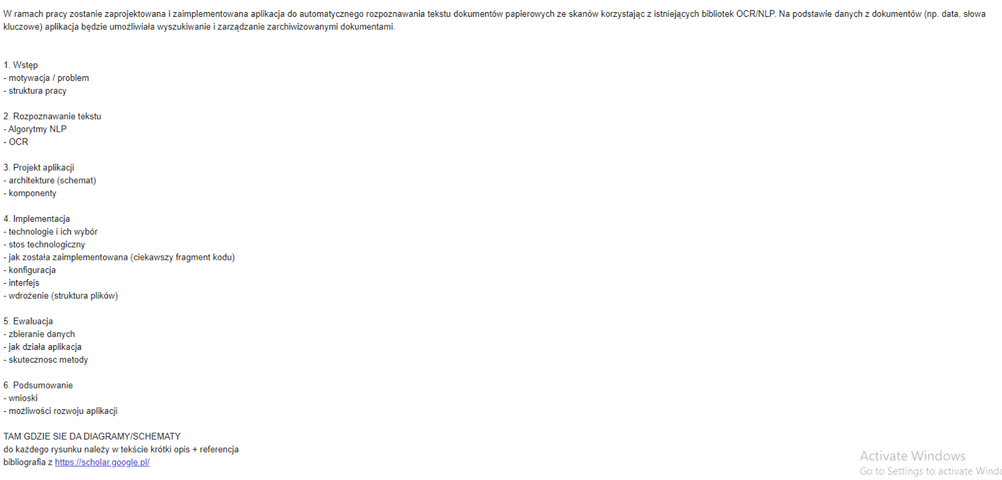
\includegraphics[width=\linewidth]{architektura.png}
	\caption{Składowe aplikacji oraz sposób ich komunikacji}
\end{figure}

\section{Autentykacja i autoryzacja}
\section{Pomost}
\section{Tworzenie ofert}
\section{Baza danych}